Throughout all of the various aggregation methods covered with and without experimentation, trying to find good ideas and sensible applications of them has been an end goal.
Ultimately, none of the robust aggregators have performed as well as I would have liked on the higher numbers of malicious clients and tend to have reduced accuracy if anything.
This lead me down the path of trying to use ideas from current aggregators and methods in federated learning to try to improve on the SotA.

\section{Clustering}
Initially, I thought about clustering similar models together through K-Means Clustering.
Similar ideas like this have been tried already \cite{cluster_robagg} but didn't really attempt anything that I would personally call robust (even if they claimed otherwise).
So, I wanted to build upon this idea by instead using some combination of FedAvg, COMED and MKRUM to do the aggregation.
I couldn't really use AFA of FedMGDA++ as they both relied on learned information about the whole system.
FedMGDA++ especially relied on having all the clients present at every step on never subsets of the clients.
\\ \\ 
However, robustly aggregating at only the clustering stage seemed like it would very easily be abused by a coordinated attack of malicious clients.
This is because malicious clients would end up having similar models due to their coordinated attack strategy being the same.
Therefore, there would always be at least one cluster of just malicious clients.
Something like COMED might be able to handle this better but it was something definitely worth investigating.
So, I would then also need to have robust aggregation happen when aggregating the cluster centres together to form the end model (something that hadn't been done before).
\\ \\
Prior to any testing, one thing that is important to bring up is that K-Means Clustering is a very computationally intensive algorithm to run.
Increasing the number of clients beyond the 30 here to systems with orders of magnitudes of more clients might not be a sustainable process.

\subsection{Aggregator Capabilities}
There are 9 different combinations of aggregators that I can try but realistically having FedAvg be the aggregator in the second aggregation step is pretty futile as malicious clients are pretty guaranteed to get through and damage the model.
Also, for trying to segregate the clients' models from each other, more training than the standard 2 epochs will need to be done.
So, I increased the number of epochs per round to 10 when we're clustering so that each client's model can appropriately represent itself before it is clustered.
\\ \\
Very early on it appeared to be apparent that using MKRUM as an external and internal aggregator proved pretty much useless.
This was because with just 1 attack, it's performance was all over the place [\ref{fig:mkrum_bad}] with any internal aggregator.
However, COMED on the other hand seemed to steam-roll right through any number of malicious clients, only starting to fail at around 22 malicious clients.
This is incredible as this outperforms any of the other robust aggregation methods tested!
\begin{figure}[htbp]
	\centering
    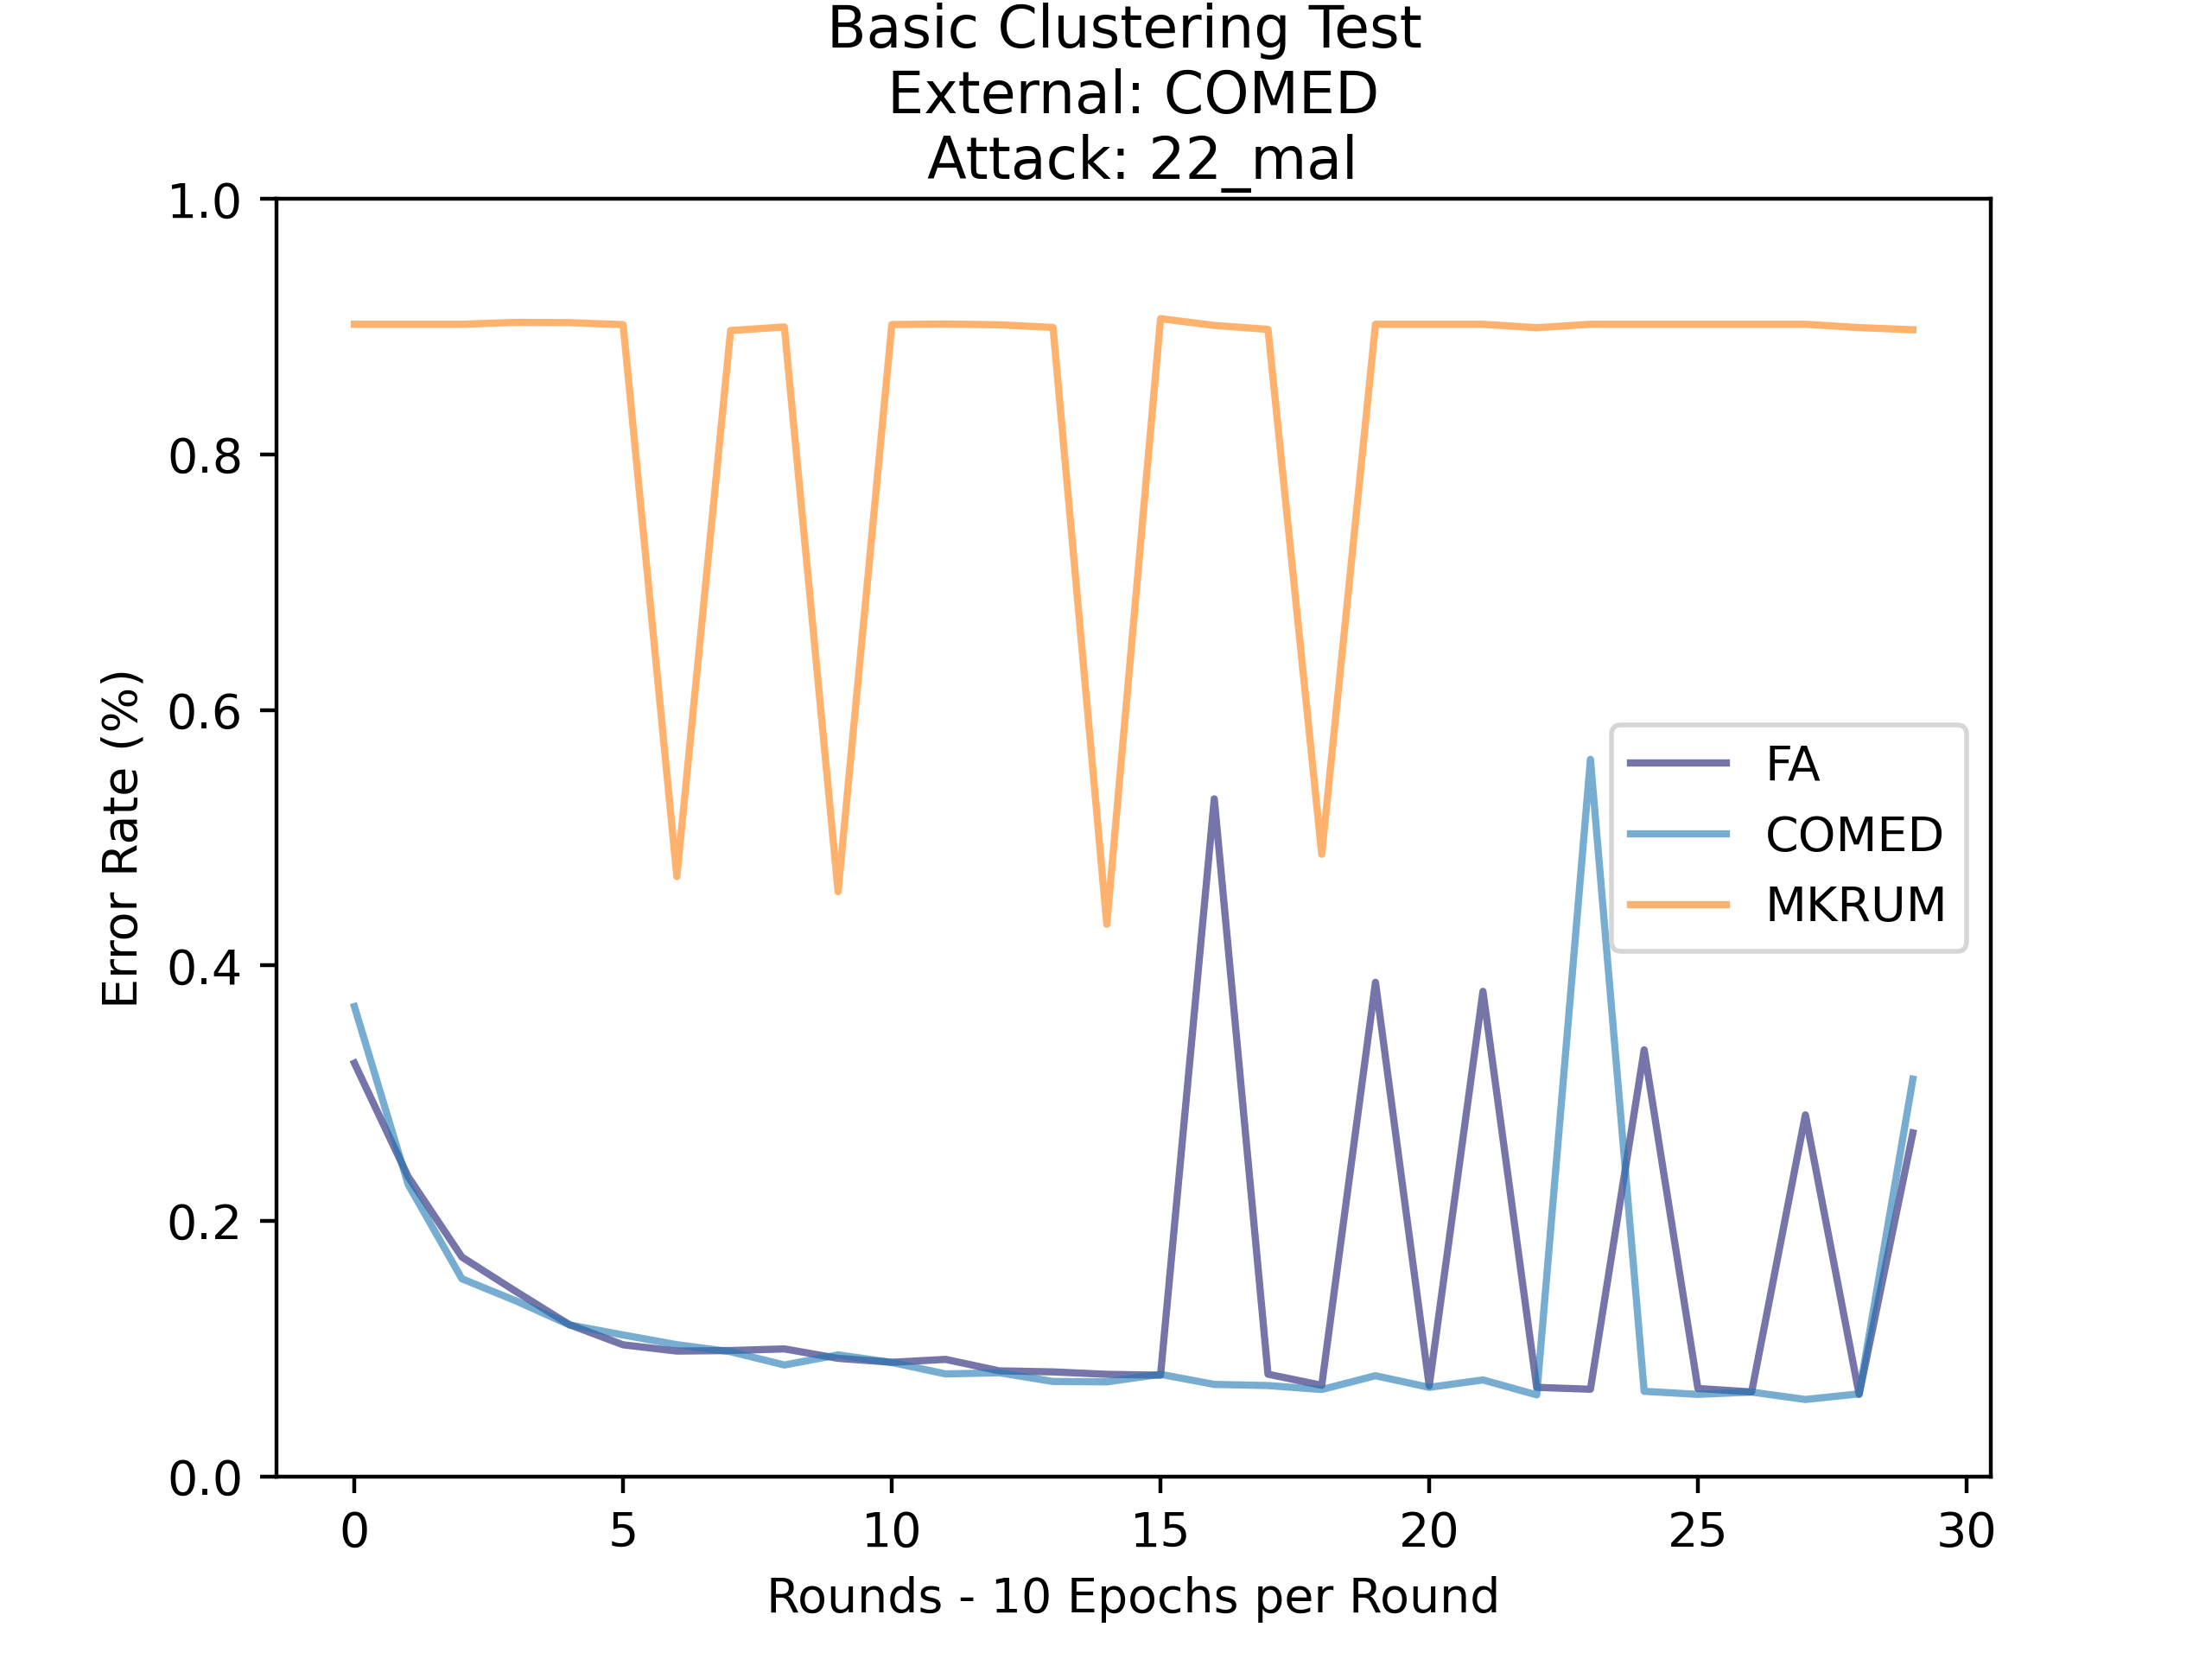
\includegraphics[scale=0.5]{my_agg/graphs/cluster_comed_22.png}
	\caption{Error Rate of K-Means Clustering with COMED as the External Aggregator - 22 Malicious Clients}
	\label{fig:comed_22}
\end{figure}
Throughout testing, both FedAvg and COMED performed similarly in their internal ability to aggregate, with it only varying later on.
One thing to note is that when the data is non-IID, it might not be as simple as that and FedAvg might start to outperform COMED through its increased data use.
\\ \\
What's also interesting to see is the extremely quick convergence of the model.
This is most likely due to no interference from the malicious clients in the first half of the total number of rounds.
You can also clearly see that the model itself is over-fitting and should realistically only be lasting for 10-15 rounds or so.
This would then help with the later stage spikes that we see.
\\ \\
It didn't quite end there though, as for some very strange reason, MKRUM's performance appeared to get better with more malicious clients being added.
This was such that I was seeing performance from MKRUM being used as an external aggregator compared to COMED at more than 22 malicious clients.
Now, this doesn't then lead me to believe that overall MKRUM performs better, just that it has its very unique and weird moments of performance.
Overall, I believe that using FedAvg to aggregate the clients within the clusters and using COMED to aggregate the cluster centres is the best way forward.


\subsection{Finding the Optimal K}
When it comes to K-Means Clustering, finding the best K-value to use is extremely important to ensure that the data is properly split up and segmented.
Luckily, it is not a particularly complex task and normally just requires testing out the different K-values and using something called the "Elbow Method" to determine which is the best.
\\ \\
The elbow method is when you plot the the number of clusters against some distance/scoring metric.
This could be their literal distance, sum of squared distances, based on accuracy etc.
In plotting there will be a more highlighted point [\ref{fig:elbow}] where the rate of change drastically decreases.
This indicates that further increases in the K-value result in not much benefit and would most likely be over-fitting the data.
\begin{figure}[htbp]
	\centering
    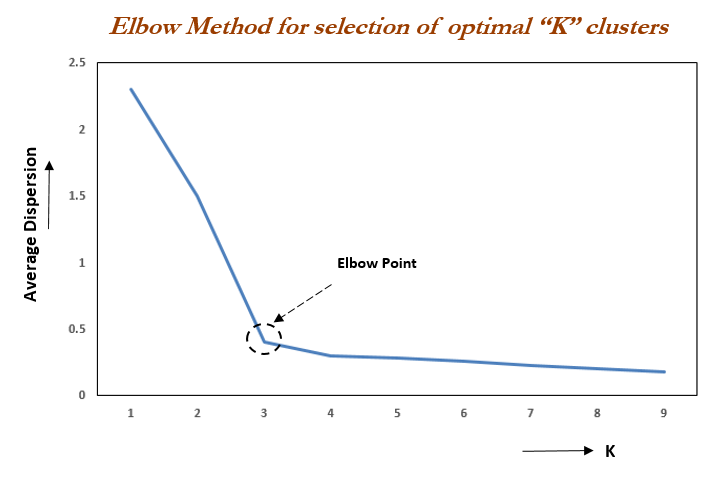
\includegraphics[scale=0.5]{my_agg/graphs/elbow.png}
	\caption{Elbow Method with Highlighted Optimal K-value \cite{oreily_elbow}}
	\label{fig:elbow}
\end{figure}
\\ \\
For the scoring metric I decided to plot the sum of the distances that each model is away from its designated cluster and total it for each value of K from 1 to 30.
Now, there are definitely less hard-coded solutions than this and ultimately using a solution that would have this K-value change would be the most ideal.
However, to recalculate this at every federated round takes minutes for even small models like with MNIST.
So, realistically trying to get a rough idea of the values of K that would be more desirable is the more sensible choice.
\\ \\
Funnily enough, there ended up not being any particular point that could be realistically identified as the elbow point.
I did the above calculations for no attacks, 5 and 20 malicious at rounds 0, 5 and 20 [\ref{fig:k_elbow}].
This was so that I was able to see how representation of the data changed throughout so I wasn't simply basing my analysis from 1 point.
\\ \\
Under no attacks, the line was a constant gradient on average and gave no hint of an optimum point.
Under 5 malicious there were similar characteristics but with a slightly steeper descent at first, potentially hinting at some K-value around 4.
At 20 malicious is where things get weird and it is almost like a K of 2 is the best.
\\ \\
Interpreting these results is interesting to say the least, but one last method I can try is to see what the final and/or minimum error rate values are at each K and see if that can shed any more light on the situation.
What I am expecting is that there won't be much difference with 0 attacks but having a good K value will be more and more important with 5 and 20 as that is where you'll see damage starting to be being done.
\begin{center}
    \begin{longtable}{ |c|c|c|c|c|c|c|c|c|c|c|c|c| }
    \caption{Error Rate (\%) as K Changes}
    \label{tbl:k_error_rate}
    \hline
    K & 1 & 2 & 3 & 4 & 5 & 6 & 7 & 8 & ... & 15 & ... & 30 \\ \hline
    \multicolumn{13}{|c|}{} \\ \hline
    0-Min & 5.3 & 7.4 & 5.7	& 5.7	& 5.4	& 5.3	& 5.3	& 5.1 & ...	& 5.4 & ... & 5.4 \\ \hline
    0-Final & 5.3	& 7.9	& 5.8	& 5.8	& 5.4	& 5.5	& 5.6	& 5.1 & ...	& 5.4 & ...  & 5.4 \\ \hline
    \multicolumn{13}{|c|}{} \\ \hline
    5-Min & 8.8 &	90.2 &	14.1 &	9.4 &	7.2 &	6.5 &	6.3 &	6.0 & ... &	5.6 & ...  & 7.3 \\ \hline
    5-Final & 28.6	& 90.2	& 16.2	& 9.4	& 7.9	& 6.5	& 6.3	& 6.0 & ...	& 5.8 & ...  & 7.5 \\ \hline
    \multicolumn{13}{|c|}{} \\ \hline
    20-Min & 90.2	& 90.2	& 13.4	& 9.4	& 7.3	& 7.4	& 6.5	& 6.4 & ...	& 25.4 & ...  & 89.7 \\ \hline
    20-Final & 90.2	& 90.2	& 16.39	& 9.82	& 8.24	& 7.4	& 6.72	& 11.9	& ...	& 26.94 & ...  & 90.2 \\ \hline
    \end{longtable}
\end{center}
Through setting the number of rounds to 15 to stop over-fitting and remove the peaks near the end, we can now see how the solutions perform at various points in Table \ref{tbl:k_error_rate}.
Seeing the no attack error rates really seemed to fit perfectly with the previous test done as the value doesn't change too much [\ref{fig:k_elbow_0}] except when K is 2.
After about the halfway point, K seems to do a little worse as well on average, indicating that it's probably become too high (although it's very minimal).
\\ \\
Where things start to change a bit is when we increase the number of malicious clients to 5.
Here, we now notice [\ref{fig:k_elbow_5}] that K has to be a minimum of 3 for the clustering to work properly.
Going any higher than 6/7 gives no improvement and would be overkill in this situation.
It should be noted that right at the very end, when the algorithm is essentially just COMED by itself, there is a gentle increase in the error rate.
\\ \\
Finally, we hit some good data with 20 malicious clients [\ref{fig:k_elbow_20}] as there is a proper U-shape to the error rate.
This further highlights that between 3 and 5 is the optimum number for K with the elbow-point being at about 3 or 4.
Noticing that the final value at K=3 is slightly higher than the minimum value suggests that the solution there is getting a bit worse nearer to the end of the federated rounds.
This leads me to conclude that a K of around 5 is the optimal for this instance but in general terms, values between 3 and 7 should probably work fine.




\section{Dimension Reduction}
When it comes to clustering the data, performing it on the entire model's parameters is very much a noisy affair as there will be plenty of parameters that aren't very important.
What we then end up with, is a clustering that relies on a bunch of noise to be performed.
For a point of reference, the MNIST model that I am using contains 535818 different parameters (with larger models getting into the millions).
Realistically, there are only going to be a certain number of parameters that are actually useful and will contribute to the clustering properly.
\\ \\
Current methods through using a VAE exist but only alongside SAD and they don't fully utilise the pure lower-dimensional form that is created and is instead used for reconstruction.
Not only this, but the hyper-parameter fine-tuning that must go into such a model (e.g. number of layers, layer size etc.) provides a more variable solution that must be curated.
They also require training to be accurate and so aren't going to be as effective early on in the aggregation.
\\ \\
However, that doesn't mean they aren't useful.
VAEs are great when you do want to reconstruct data (and maybe compare that way) but ultimately that is not the goal that I am trying to achieve here.
This is where Principal Component Analysis (PCA) comes in.
PCA is a quick and effective form of dimensionality reduction that can create a more concise representation of our models.

\subsection{Number of Dimensions}
The only parameter that can really be chosen for PCA is what dimension should the data be represented in.
We could perform similar tests that were done for K-Means but luckily PCA provides a handy little thing called "Explained Variance".
This is essentially just sum of squared distances but in more mathematical terms it is used to measure discrepancies between the representation via PCA and the actual data.
This works very nicely for us as we want to keep as much useful information as possible without over-fitting.
\begin{figure}[htbp]
	\centering
    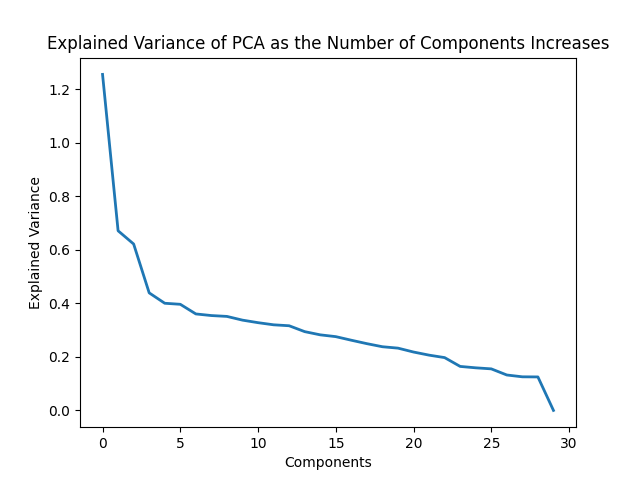
\includegraphics[scale=0.5]{my_agg/graphs/0_r0.png}
	\caption{Explained Variance with No Attacks at Round 0}
	\label{fig:pca_00}
\end{figure}
\\ \\
As seen in [\ref{fig:pca_00}], we can start to see that a dimension value of around 1-4 is probably the sweet spot.
Other rounds later on [\ref{fig:pca_01}, \ref{fig:pca_02}] may appear to indicate that actually we don't want to perform PCA at all.
However, this pattern only really appears when there are no attacks present and as soon as we start adding some, it becomes more apparent [\ref{fig:pca_50}] that this is not the case.
Instead, we end up seeing that a dimension value of 1 looks to be a pretty safe bet with some potential at round 2-4.


\subsection{Low Dimensional Beings}
As has become apparent, relying on traditional methods to guarantee what the optimal values are, is not always the best idea.
So, to help further guarantee that the low PCA dimension values are correct, let's plot the coordinates of these values and see how they compare.
We can only do this in 1D, 2D, 3D and 4D but seeing as it theoretically shouldn't need to go beyond this anyway, it should be fine.
\\ \\





\section{Personalisation}






\section{Bringing it All Together}




